\documentclass[twoside]{book}

% Packages required by doxygen
\usepackage{fixltx2e}
\usepackage{calc}
\usepackage{doxygen}
\usepackage[export]{adjustbox} % also loads graphicx
\usepackage{graphicx}
\usepackage[utf8]{inputenc}
\usepackage{makeidx}
\usepackage{multicol}
\usepackage{multirow}
\PassOptionsToPackage{warn}{textcomp}
\usepackage{textcomp}
\usepackage[nointegrals]{wasysym}
\usepackage[table]{xcolor}

% Font selection
\usepackage[T1]{fontenc}
\usepackage[scaled=.90]{helvet}
\usepackage{courier}
\usepackage{amssymb}
\usepackage{sectsty}
\renewcommand{\familydefault}{\sfdefault}
\allsectionsfont{%
  \fontseries{bc}\selectfont%
  \color{darkgray}%
}
\renewcommand{\DoxyLabelFont}{%
  \fontseries{bc}\selectfont%
  \color{darkgray}%
}
\newcommand{\+}{\discretionary{\mbox{\scriptsize$\hookleftarrow$}}{}{}}

% Page & text layout
\usepackage{geometry}
\geometry{%
  a4paper,%
  top=2.5cm,%
  bottom=2.5cm,%
  left=2.5cm,%
  right=2.5cm%
}
\tolerance=750
\hfuzz=15pt
\hbadness=750
\setlength{\emergencystretch}{15pt}
\setlength{\parindent}{0cm}
\setlength{\parskip}{3ex plus 2ex minus 2ex}
\makeatletter
\renewcommand{\paragraph}{%
  \@startsection{paragraph}{4}{0ex}{-1.0ex}{1.0ex}{%
    \normalfont\normalsize\bfseries\SS@parafont%
  }%
}
\renewcommand{\subparagraph}{%
  \@startsection{subparagraph}{5}{0ex}{-1.0ex}{1.0ex}{%
    \normalfont\normalsize\bfseries\SS@subparafont%
  }%
}
\makeatother

% Headers & footers
\usepackage{fancyhdr}
\pagestyle{fancyplain}
\fancyhead[LE]{\fancyplain{}{\bfseries\thepage}}
\fancyhead[CE]{\fancyplain{}{}}
\fancyhead[RE]{\fancyplain{}{\bfseries\leftmark}}
\fancyhead[LO]{\fancyplain{}{\bfseries\rightmark}}
\fancyhead[CO]{\fancyplain{}{}}
\fancyhead[RO]{\fancyplain{}{\bfseries\thepage}}
\fancyfoot[LE]{\fancyplain{}{}}
\fancyfoot[CE]{\fancyplain{}{}}
\fancyfoot[RE]{\fancyplain{}{\bfseries\scriptsize Generated by Doxygen }}
\fancyfoot[LO]{\fancyplain{}{\bfseries\scriptsize Generated by Doxygen }}
\fancyfoot[CO]{\fancyplain{}{}}
\fancyfoot[RO]{\fancyplain{}{}}
\renewcommand{\footrulewidth}{0.4pt}
\renewcommand{\chaptermark}[1]{%
  \markboth{#1}{}%
}
\renewcommand{\sectionmark}[1]{%
  \markright{\thesection\ #1}%
}

% Indices & bibliography
\usepackage{natbib}
\usepackage[titles]{tocloft}
\setcounter{tocdepth}{3}
\setcounter{secnumdepth}{5}
\makeindex

% Custom commands
\newcommand{\clearemptydoublepage}{%
  \newpage{\pagestyle{empty}\cleardoublepage}%
}

\usepackage{caption}
\captionsetup{labelsep=space,justification=centering,font={bf},singlelinecheck=off,skip=4pt,position=top}

%===== C O N T E N T S =====

\begin{document}

% Titlepage & ToC
\pagenumbering{roman}
\begin{titlepage}
\vspace*{7cm}
\begin{center}%
{\Large Practica 1 Actividad 2 }\\
\vspace*{1cm}
{\large Generated by Doxygen 1.8.11}\\
\end{center}
\end{titlepage}
\clearemptydoublepage
\tableofcontents
\clearemptydoublepage
\pagenumbering{arabic}

%--- Begin generated contents ---
\chapter{Hierarchical Index}
\section{Class Hierarchy}
This inheritance list is sorted roughly, but not completely, alphabetically\+:\begin{DoxyCompactList}
\item \contentsline{section}{Client}{\pageref{class_client}}{}
\item Remote\begin{DoxyCompactList}
\item \contentsline{section}{Client\+\_\+\+Server}{\pageref{interface_client___server}}{}
\begin{DoxyCompactList}
\item \contentsline{section}{Server}{\pageref{class_server}}{}
\end{DoxyCompactList}
\end{DoxyCompactList}
\end{DoxyCompactList}

\chapter{Class Index}
\section{Class List}
Here are the classes, structs, unions and interfaces with brief descriptions\+:\begin{DoxyCompactList}
\item\contentsline{section}{{\bf main} }{\pageref{classmain}}{}
\item\contentsline{section}{{\bf Matrix} \\*\doxyref{Matrix}{p.}{class_matrix} class to create and control a integer matrix.  public }{\pageref{class_matrix}}{}
\end{DoxyCompactList}

\chapter{File Index}
\section{File List}
Here is a list of all files with brief descriptions\+:\begin{DoxyCompactList}
\item\contentsline{section}{C\+:/\+Users/\+Alfredo/workspace/\+P\+\_\+3/src/{\bf A.\+java} }{\pageref{_a_8java}}{}
\item\contentsline{section}{C\+:/\+Users/\+Alfredo/workspace/\+P\+\_\+3/src/{\bf B.\+java} }{\pageref{_b_8java}}{}
\item\contentsline{section}{C\+:/\+Users/\+Alfredo/workspace/\+P\+\_\+3/src/{\bf Contador.\+java} }{\pageref{_contador_8java}}{}
\item\contentsline{section}{C\+:/\+Users/\+Alfredo/workspace/\+P\+\_\+3/src/{\bf main.\+java} }{\pageref{main_8java}}{}
\end{DoxyCompactList}

\chapter{Class Documentation}
\section{main Class Reference}
\label{classmain}\index{main@{main}}
\subsection*{Static Public Member Functions}
\begin{DoxyCompactItemize}
\item 
static void {\bf main} (String[$\,$] args)  throws Exception 
\begin{DoxyCompactList}\small\item\em Method Main of the project, where other programs are initialized. \end{DoxyCompactList}\end{DoxyCompactItemize}


\subsection{Constructor \& Destructor Documentation}
\index{main@{main}!main@{main}}
\index{main@{main}!main@{main}}
\subsubsection[{main(\+String[] args)}]{\setlength{\rightskip}{0pt plus 5cm}static void main.\+main (
\begin{DoxyParamCaption}
\item[{String[$\,$]}]{args}
\end{DoxyParamCaption}
) throws Exception\hspace{0.3cm}{\ttfamily [static]}}\label{classmain_a0877f3b412d48b8c92fa25c4b98c2f5a}


Method Main of the project, where other programs are initialized. 


\begin{DoxyParams}{Parameters}
{\em args} & \\
\hline
\end{DoxyParams}

\begin{DoxyExceptions}{Exceptions}
{\em Exception} & \\
\hline
\end{DoxyExceptions}
\begin{DoxyReturn}{Returns}
void  public static 
\end{DoxyReturn}


The documentation for this class was generated from the following file\+:\begin{DoxyCompactItemize}
\item 
src/{\bf main.\+java}\end{DoxyCompactItemize}

\section{Matrix Class Reference}
\label{class_matrix}\index{Matrix@{Matrix}}


\doxyref{Matrix}{p.}{class_matrix} class to create and control a integer matrix.  public.  


Inheritance diagram for Matrix\+:\begin{figure}[H]
\begin{center}
\leavevmode
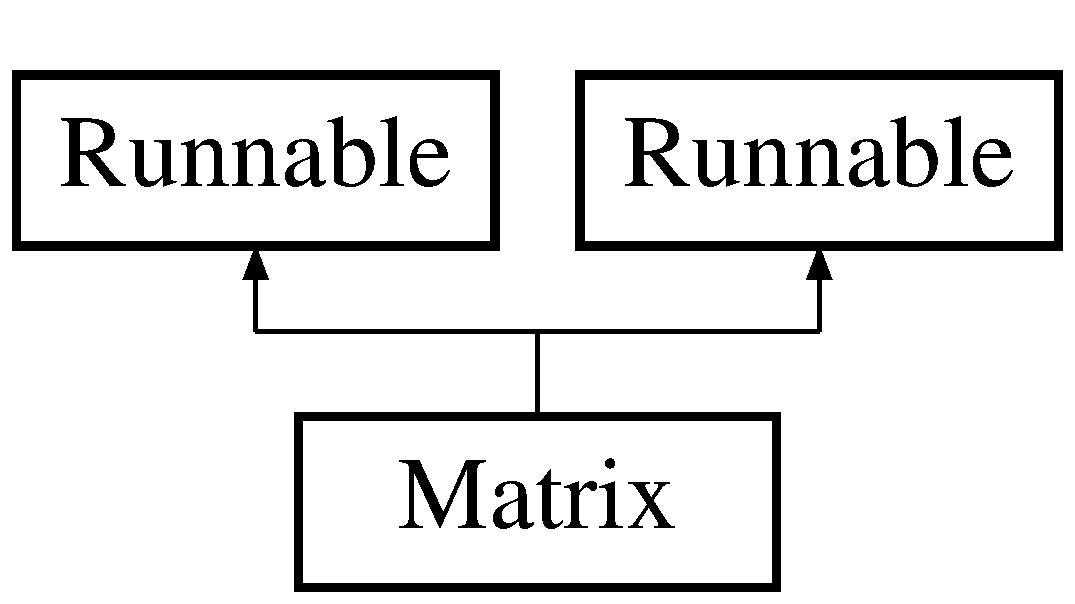
\includegraphics[height=2.000000cm]{class_matrix}
\end{center}
\end{figure}
\subsection*{Public Member Functions}
\begin{DoxyCompactItemize}
\item 
{\bf Matrix} (int n)
\begin{DoxyCompactList}\small\item\em \doxyref{Matrix}{p.}{class_matrix} constructor, sets the matrix dimension and creates the integer matrix. \end{DoxyCompactList}\item 
{\bf Matrix} (int t, int a)
\begin{DoxyCompactList}\small\item\em \doxyref{Matrix}{p.}{class_matrix} constructor, sets the type and the Threads amount. \end{DoxyCompactList}\item 
int {\bf get\+Max\+Elem} ()
\begin{DoxyCompactList}\small\item\em Get max element. \end{DoxyCompactList}\item 
void {\bf set\+Max\+Elem} (int e)
\begin{DoxyCompactList}\small\item\em Set max element. \end{DoxyCompactList}\item 
int {\bf get\+Elem} (int p)  throws Exception
\begin{DoxyCompactList}\small\item\em Get element in a position. \end{DoxyCompactList}\item 
void {\bf set\+Elem} (int e)
\begin{DoxyCompactList}\small\item\em Set element. \end{DoxyCompactList}\item 
int {\bf get\+Amount} ()
\begin{DoxyCompactList}\small\item\em Get amount. \end{DoxyCompactList}\item 
synchronized boolean {\bf is\+Full} ()
\begin{DoxyCompactList}\small\item\em Check if the matrix is full. \end{DoxyCompactList}\item 
void {\bf fill\+Matrix} ()
\begin{DoxyCompactList}\small\item\em Sets random element to the integer matrix. \end{DoxyCompactList}\item 
void {\bf show\+Matrix} ()
\begin{DoxyCompactList}\small\item\em Show the matrix in the screen. \end{DoxyCompactList}\item 
void {\bf add\+Matrix} ({\bf Matrix} a, {\bf Matrix} b, boolean threads)  throws Exception
\begin{DoxyCompactList}\small\item\em Sets the integer matrix, adding the value of two elements from another matrices. \end{DoxyCompactList}\item 
void {\bf run} ()
\end{DoxyCompactItemize}


\subsection{Detailed Description}
\doxyref{Matrix}{p.}{class_matrix} class to create and control a integer matrix.  public. 

\subsection{Constructor \& Destructor Documentation}
\index{Matrix@{Matrix}!Matrix@{Matrix}}
\index{Matrix@{Matrix}!Matrix@{Matrix}}
\subsubsection[{Matrix(int n)}]{\setlength{\rightskip}{0pt plus 5cm}Matrix.\+Matrix (
\begin{DoxyParamCaption}
\item[{int}]{n}
\end{DoxyParamCaption}
)}\label{class_matrix_abb538ba5e460548bfa8e9f81716d5fe9}


\doxyref{Matrix}{p.}{class_matrix} constructor, sets the matrix dimension and creates the integer matrix. 


\begin{DoxyParams}{Parameters}
{\em int} & n  public \\
\hline
\end{DoxyParams}
\index{Matrix@{Matrix}!Matrix@{Matrix}}
\index{Matrix@{Matrix}!Matrix@{Matrix}}
\subsubsection[{Matrix(int t, int a)}]{\setlength{\rightskip}{0pt plus 5cm}Matrix.\+Matrix (
\begin{DoxyParamCaption}
\item[{int}]{t, }
\item[{int}]{a}
\end{DoxyParamCaption}
)}\label{class_matrix_addba9b5fb6448b716ca95f3e803c9e97}


\doxyref{Matrix}{p.}{class_matrix} constructor, sets the type and the Threads amount. 


\begin{DoxyParams}{Parameters}
{\em int} & t, int a  public \\
\hline
\end{DoxyParams}


\subsection{Member Function Documentation}
\index{Matrix@{Matrix}!add\+Matrix@{add\+Matrix}}
\index{add\+Matrix@{add\+Matrix}!Matrix@{Matrix}}
\subsubsection[{add\+Matrix(\+Matrix a, Matrix b, boolean threads)}]{\setlength{\rightskip}{0pt plus 5cm}void Matrix.\+add\+Matrix (
\begin{DoxyParamCaption}
\item[{{\bf Matrix}}]{a, }
\item[{{\bf Matrix}}]{b, }
\item[{boolean}]{threads}
\end{DoxyParamCaption}
) throws Exception}\label{class_matrix_a35a2d6ea3fe8026cf6f3c23309fc702a}


Sets the integer matrix, adding the value of two elements from another matrices. 


\begin{DoxyParams}{Parameters}
{\em \doxyref{Matrix}{p.}{class_matrix}} & a, \doxyref{Matrix}{p.}{class_matrix} b,boolean threads \\
\hline
\end{DoxyParams}
\begin{DoxyReturn}{Returns}
void 
\end{DoxyReturn}

\begin{DoxyExceptions}{Exceptions}
{\em Exception} & public \\
\hline
\end{DoxyExceptions}
\index{Matrix@{Matrix}!fill\+Matrix@{fill\+Matrix}}
\index{fill\+Matrix@{fill\+Matrix}!Matrix@{Matrix}}
\subsubsection[{fill\+Matrix()}]{\setlength{\rightskip}{0pt plus 5cm}void Matrix.\+fill\+Matrix (
\begin{DoxyParamCaption}
{}
\end{DoxyParamCaption}
)}\label{class_matrix_a109ca8521a53d4cc0d3a799bdcfa479f}


Sets random element to the integer matrix. 

\begin{DoxyReturn}{Returns}
void  public 
\end{DoxyReturn}
\index{Matrix@{Matrix}!get\+Amount@{get\+Amount}}
\index{get\+Amount@{get\+Amount}!Matrix@{Matrix}}
\subsubsection[{get\+Amount()}]{\setlength{\rightskip}{0pt plus 5cm}int Matrix.\+get\+Amount (
\begin{DoxyParamCaption}
{}
\end{DoxyParamCaption}
)}\label{class_matrix_ad4e58f60b35a9730db60ce2fea6a113a}


Get amount. 

\begin{DoxyReturn}{Returns}
integer  public 
\end{DoxyReturn}
\index{Matrix@{Matrix}!get\+Elem@{get\+Elem}}
\index{get\+Elem@{get\+Elem}!Matrix@{Matrix}}
\subsubsection[{get\+Elem(int p)}]{\setlength{\rightskip}{0pt plus 5cm}int Matrix.\+get\+Elem (
\begin{DoxyParamCaption}
\item[{int}]{p}
\end{DoxyParamCaption}
) throws Exception}\label{class_matrix_a15560c5ba875df98d212243dcecf50eb}


Get element in a position. 


\begin{DoxyParams}{Parameters}
{\em int} & p \\
\hline
\end{DoxyParams}
\begin{DoxyReturn}{Returns}
integer 
\end{DoxyReturn}

\begin{DoxyExceptions}{Exceptions}
{\em Exception} & public \\
\hline
\end{DoxyExceptions}
\index{Matrix@{Matrix}!get\+Max\+Elem@{get\+Max\+Elem}}
\index{get\+Max\+Elem@{get\+Max\+Elem}!Matrix@{Matrix}}
\subsubsection[{get\+Max\+Elem()}]{\setlength{\rightskip}{0pt plus 5cm}int Matrix.\+get\+Max\+Elem (
\begin{DoxyParamCaption}
{}
\end{DoxyParamCaption}
)}\label{class_matrix_ae770376be5cec1a902e88a12d1d19430}


Get max element. 

\begin{DoxyReturn}{Returns}
integer  public 
\end{DoxyReturn}
\index{Matrix@{Matrix}!is\+Full@{is\+Full}}
\index{is\+Full@{is\+Full}!Matrix@{Matrix}}
\subsubsection[{is\+Full()}]{\setlength{\rightskip}{0pt plus 5cm}synchronized boolean Matrix.\+is\+Full (
\begin{DoxyParamCaption}
{}
\end{DoxyParamCaption}
)}\label{class_matrix_a0f9e6d3a21091bc2372b50e2c531f380}


Check if the matrix is full. 

\begin{DoxyReturn}{Returns}
boolean  public 
\end{DoxyReturn}
\index{Matrix@{Matrix}!run@{run}}
\index{run@{run}!Matrix@{Matrix}}
\subsubsection[{run()}]{\setlength{\rightskip}{0pt plus 5cm}void Matrix.\+run (
\begin{DoxyParamCaption}
{}
\end{DoxyParamCaption}
)}\label{class_matrix_ad0983faaafd3fc1f5b0b5a4ad0be3146}
Run function. Running to start the thread. \begin{DoxyReturn}{Returns}
void  public 
\end{DoxyReturn}
\index{Matrix@{Matrix}!set\+Elem@{set\+Elem}}
\index{set\+Elem@{set\+Elem}!Matrix@{Matrix}}
\subsubsection[{set\+Elem(int e)}]{\setlength{\rightskip}{0pt plus 5cm}void Matrix.\+set\+Elem (
\begin{DoxyParamCaption}
\item[{int}]{e}
\end{DoxyParamCaption}
)}\label{class_matrix_acf6368a332a81a1f9fcf93c104b8aa36}


Set element. 


\begin{DoxyParams}{Parameters}
{\em int} & e \\
\hline
\end{DoxyParams}
\begin{DoxyReturn}{Returns}
void  public 
\end{DoxyReturn}
\index{Matrix@{Matrix}!set\+Max\+Elem@{set\+Max\+Elem}}
\index{set\+Max\+Elem@{set\+Max\+Elem}!Matrix@{Matrix}}
\subsubsection[{set\+Max\+Elem(int e)}]{\setlength{\rightskip}{0pt plus 5cm}void Matrix.\+set\+Max\+Elem (
\begin{DoxyParamCaption}
\item[{int}]{e}
\end{DoxyParamCaption}
)}\label{class_matrix_adbd750f2d2b6298cacd867e5c1a241f5}


Set max element. 


\begin{DoxyParams}{Parameters}
{\em int} & e \\
\hline
\end{DoxyParams}
\begin{DoxyReturn}{Returns}
void  public 
\end{DoxyReturn}
\index{Matrix@{Matrix}!show\+Matrix@{show\+Matrix}}
\index{show\+Matrix@{show\+Matrix}!Matrix@{Matrix}}
\subsubsection[{show\+Matrix()}]{\setlength{\rightskip}{0pt plus 5cm}void Matrix.\+show\+Matrix (
\begin{DoxyParamCaption}
{}
\end{DoxyParamCaption}
)}\label{class_matrix_a2e244df6046157de788a026a54fed620}


Show the matrix in the screen. 

\begin{DoxyReturn}{Returns}
void  public 
\end{DoxyReturn}


The documentation for this class was generated from the following file\+:\begin{DoxyCompactItemize}
\item 
src/{\bf Matrix.\+java}\end{DoxyCompactItemize}

\chapter{File Documentation}
\section{C\+:/\+Users/\+Alfredo/workspace/\+P\+\_\+3/src/main.java File Reference}
\label{main_8java}\index{C\+:/\+Users/\+Alfredo/workspace/\+P\+\_\+3/src/main.\+java@{C\+:/\+Users/\+Alfredo/workspace/\+P\+\_\+3/src/main.\+java}}
\subsection*{Classes}
\begin{DoxyCompactItemize}
\item 
class {\bf main}
\end{DoxyCompactItemize}

\section{src/\+Matrix.java File Reference}
\label{_matrix_8java}\index{src/\+Matrix.\+java@{src/\+Matrix.\+java}}
\subsection*{Classes}
\begin{DoxyCompactItemize}
\item 
class {\bf Matrix}
\begin{DoxyCompactList}\small\item\em \doxyref{Matrix}{p.}{class_matrix} class to create and control a integer matrix.  public. \end{DoxyCompactList}\end{DoxyCompactItemize}

%--- End generated contents ---

% Index
\backmatter
\newpage
\phantomsection
\clearemptydoublepage
\addcontentsline{toc}{chapter}{Index}
\printindex

\end{document}
